\documentclass[a4paper,10pt]{scrartcl}
\usepackage{mathe-vorlesung}
\usepackage{graphicx}
\renewcommand{\equiv}{\Longleftrightarrow}
\newcommand{\eps}{\varepsilon}
\newcommand{\del}{\delta}

\title{Physik Vorkurs}

\begin{document}

\maketitle

\tableofcontents
\newpage
\begin{center}
\LARGE\textbf{Vorwort}
\end{center}
\begin{seg}{Was ist Topologie?}
\begin{itemize}
\item "` Unterzeichnung geometrischer Objekte bis auf stetige Dekorationen. "'
\item "` Stetigkeitsgeometrie"', "` qualitative Geometrie "', "`Gummi-Geometrie"'
\end{itemize}
Objekte werden in der Topologie als gleich angesehen, wenn sie durch eine in beiden Richtungen stetige bijektive Abbildung aufeinander abgebildet werden kann ("` Homöomorphismus"').
\end{seg}
So zum Beispiel für Teilmengen des $\R^2$:
\begin{figure}[h]
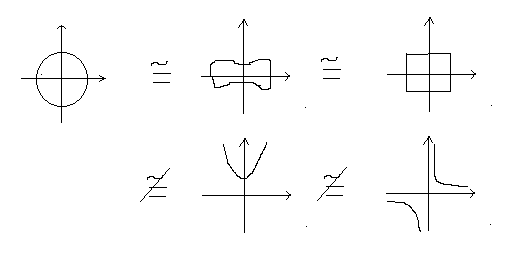
\includegraphics[scale=0.7]{fig1.png}
\end{figure}
\begin{ex*} 
Topologische Begriffe sind beispielsweise \emph{Stetigkeit, offene/abgeschlossene Mengen, Umgebung, Rand, Abschluss, Konvergenz, kompakt, zusammenhängend, Homotopie}.  Die konkreten Definition werden im Verlauf dieser Vorlesung geklärt.
\end{ex*}
\begin{center}
\LARGE\textbf{I Grundbegriffe}
\end{center}
\section{Metrische und topologische Räume}
\begin{df}
Ein \emph{metrischer Raum} ist eine Menge $X$k zusammen mit einer Funktion $d: X \times X \rightarrow \R$, genannt Metrik oder \emph{Abstandsfunktion}, so dass folgende Axiome gelten:
\begin{enumerate}[\roman{enumi})]
\item \emph{Positivität}: $d(x,y)\ge 0 \land d(x,y)=0\equiv x=y$
\item \emph{Symmetrie}: $d(x,y)=d(y,x)$
\item \emph{Dreiecksungleichung}: $d(x,z) \le d(x,y)+d(y,z)$
\end{enumerate}
\end{df}
\begin{ex*}
Auf $\R^n$ ist durch die \emph{Euklidische Norm} $|x|=\sqrt{x_1^2+...+x_n^2}$ die \emph{Euklidische Abstandsfunktion} $d(x,y)=||x-y||$ gegeben. Auf $\R$ oder auf $\C$ ist diese Metrik durch den Betrag $d(x,y):=|x-y|$ definiert.  Man erhält auf diese Weise aus jeder Norm eine Metrik. Hierbei liefern verschiedene Normen natürlich verschiedene Metriken. Hier einige Beispiele auf $\R^2$:
\begin{itemize} 
\item euklidische Norm: $||x||_2=\sqrt{x_1^2+x_2^2}$
\item Maximumsnorm: $||x||_\infty := \max(|x_1|, |x_2|)$
\item $\Eins$-Norm $||x||_1 := |x_1|+|x_2|$
\end{itemize}
\end{ex*}

\begin{ex*}
Die diskrete Metrik definiert durch:
\[
d(x,y)=\begin{cases}
  0, & \text{falls} x=y \\ 1, & \text{falls} x\neq y
\end{cases}
\]
\end{ex*}

Es lassen sich zwei zentrale mathematische Begriffe mit HIlfe von Abstandsfunktionen definieren:
\begin{itemize}
\item Konvergenz von Folgen
\item Stetigkeit von Abbildungen
\end{itemize}

\begin{df}[Konvergenz im metrischen Räumen]
Sei $X$ ein metrischer Raum und $x_N, n\in \N$ eine Folge in $X$. Wir sagen $(x_n)_{n\in \N}$ \emph{konvergiert}, falls es ein $a \in X$ gibt, so dass gilt:
\[
\forall_{\varepsilon>0}\exists_{k\in\N}\forall_{n\ge k}: d(x_n,a)<\varepsilon
\]
\end{df}
In diesem Fall sagen wir, $a$ ist der \emph{Limes} (oder Grenzwert) von $(x_n)_{n\in \N}$ (und schreiben $x_n\rightarrow a, \lim\limits_{n\rightarrow \infty} x_n=a$) 

\begin{st} In einem metrischen Raum ist der Limes eine konvergente Folge eindeutig bestimmt.
\end{st}
\begin{proof}
Seien $a$ und $b$ Limiten von $(x_n)_{n\in \N}$ mit $\delta := d(a,b)>0$.

Da $(x_n)_{n\in \N}$ gegen $a$ konvergiert, gibt es $k\in \N$, sodass $d(x_n,a)<\frac{\delta}{2}$ für alle $n \ge k$.
Dann gilt nach Dreiecksungleichung:
\[
\delta=d(a,b)\le \underbrace{d(x,x_n)}_{<\frac{delta}{2}}+d(x_n,b)
\]
Also gilt $d(x_n,b)\ge \frac{\delta}{2}$ für alle $n\ge b$, was der Konvergenz gegen $b$ widerspricht.
\end{proof}
\begin{df}[$\eps$-$\delta$-Definition der Stetigkeit in metrischen Räumen]
Seien $X$ und $\tilde X$ metrische Räume mit Abstandsfunktion $d$ bzw. $\tilde d$. Eine Abbildung $f: X \rightarrow \tilde X$ heißt stetig in$x \in X$ falls gilt: 
\[\forall_{\eps>0}\exists_{\delta>0} \forall_{x'\in X}: d(x,x')<\delta \implies \tilde d(f(x), f(x'))<\eps\]

Die Abbildung heißt \emph{stetig}, falls dies für alle $x\in X$ gilt.  Stetigkeit in metrischen Räumen hängen eng zusammen. Es gilt:
\end{df}
\begin{st}
Eine Abbildung $f: X\rightarrow \tilde X$ zwischen metrischen Räume ist genau dann stetig, wenn für jede konvergente Folge $x_n \rightarrow a$ in X gilt, dass $f(x_n) \rightarrow f(a)$
\end{st} 
\begin{proof}
\begin{seg}{"`$\implies$"'}
Sei $\eps>0$, dann gibt es $\delta>0$, so dass aus $d(x',a)<\delta$ folgt: $d(f(x'),f(a))<\eps$. Weiter gibt es ein $k\in \N$, so dass $d(x_N,a)y\delta$ für $n \ge k$.  Insgesamt folgt $d(f(x_n),f(a))<\eps$ für alle $n\ge k$.
\end{seg}
\begin{seg}{"`$\Longleftarrow$"'}
Angenommen, $f$ ist nicht stetig. Dann gibt es ein $x \in X$ und ein $\eps>0$, so dass es zu jeden $n\in \N$ ein $x$ mit $d(x_n,x)<\frac{1}{n}$ und $d(f(x_1), f(x))\ge \eps$ gibt. Damit ergibt sich der Widerspruch.
\end{seg}
\end{proof}
Die obigen Definition lassen sich mit Hilfe von $\eps$-Bällen umformulieren:
\begin{df}
Sei $X$ ein metrischer Raum und $x\in X$, dann heißt die Teilmenge 
\[
B_\eps(x)={x'\in X|d(x',x)<\eps}
\]
von $X$ heißt der (\emph{offene}) \emph{Ball mit Radius $\eps$ um x} (kurz: \emph{$\eps$-Ball}).
\end{df}
\begin{df}
In einem metrischen Raum heißt eine Teilmenge $U\subset X$ \emph{offen}, wenn es um jeden ihrer Punkte einen offenen $\eps$-Ball gibt, der ganz in U enthalten. Eine Teilmenge A heißt \emph{abgeschlossen}, wenn ihr Komplement $X\setminus A$ offen ist.  Eine Teilmenge $U \subset Y$ heißt \emph{Umgebung} eines Punktes $ x\in X$, falls es eine offene Teilmenge $V \subset X$ gibt mit $x\in v$ und $V \subset U$.  (Äquivalent: falls es ein $\eps$ mit $B_\eps(x)\subset U$ gibt.  
\end{df}

\begin{figure}[h]
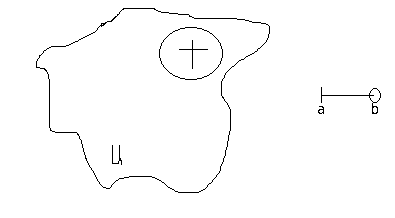
\includegraphics[scale=0.5]{fig3.png}
\end{figure}

Konvergenz und Stetigkeit lassen sich in metrischen Räumen durch offene Mengen beschreiben.
\begin{st}
In einem metrischen raum konvvergiert eine Folge $(x_n)_{n \in \N}$ genau dann gegen x, wenn es zu jeder Umgebung $U$ von $x$ ein $k \in \N$ gibt, so dass $x_n \in U$ für alle $n \ge k $ gilt.\\
\underline{Kurz:} Eine Folge $(x_n)_{n \in \N}$ konvergiert gegen $x$, wenn in jeder Umgebunng von $x$ \emph{fast alle} ($\hat =$ alle bis auf endlich viele) Folgenglieder liegen.
\end{st}
\begin{proof}
Die Äwuivalenz gilt, da jede Umgebung von $x$ einen $\eps$-Ball um $x$ enthält und umgekehrt jeden $\eps$-Ball um $x$ auch eine Umgebung von $x$ ist.
\end{proof}
\begin{st}\label{st:1.8}
Eine Abbildung zwischen metrischen Räumen $f: X\rightarrow \tilde X$ ist genau dann stetig in $x \in X$, wenn es zu jeder Umgebung $V$ von $f(X)$ eine Umgebung $U$ von $x$ gibt, so dass U unter $ f $ in V abgebildet wird; oder äquivalent dazu, falls das Urbild jeder Umgebung von $  f(x) $ eine Umgebung von x ist.
\end{st}
\begin{proof}
Dies folgt direkt aus der $ \eps $-$ \delta $-Definition der Stetigkeit und er Definition der Umgebung.
\begin{figure}[h]

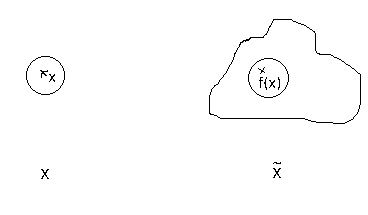
\includegraphics[scale=0.5]{fig4.png}
\end{figure}
\end{proof}
\begin{st}
Eine Abbildung zwischen metrischen Räumen ist stetig genau dann, wenn die Urbilder offener Mengen offen sind.
\end{st}
\begin{proof}
\begin{seg}{"`$\Longrightarrow$"'}
Sei $ f: X \to \tilde X $ stetig und $ V \subset \tilde Y $ offen.  Dann ist $ f^{-1}(V) $ nach \ref{st:1.8} eine Umgebung jeder ihrer Punkte somit offen.
\end{seg}
\begin{seg}{"`$\Longleftarrow$"'}
Seien umgekehrt die Urbilder offener Mengen offen und $ x \in X $. Sei $ \eps>0 $.  Nach Voraussetuuimg $ f^{-1}(B_\eps(f(x)) $ offen und enthält somit einen $ \delta $-Ball um den Punkt x.
\end{seg}
\end{proof}

Wichtige Beobachtung: Um KOnvergenz und Stetigkeit zu beschreiben muss man nicht direkt auf eine Metrik Bezug nehmen, sondern es genügt das System der offenen Mengen zu kennen.  Dieses System von offenen Mengen nennt man \emph{die Topologie} des metrischen Raums .  Verschiedene Metriken können dieselbe Topologie erzeugen.

Alle Eigenschaften von metrischen Räumen, ihren Teilmengen oder Abbildung zwischen metrischen Räumen, die sich durch die Topologie (ohne direkten Bezug auf die metrik) beschreiben lassen, nennen wir \emph{topologische Eigenschaften}.

Dies führt zu dem folgenden Begriff:
\begin{df}
Sei $ X $ eine Menge und $O \in \mathcal P (x)$ eine Menge von Teilmengen von X; $ O $ heißt eine \emph{Topologie} auf $ X $, wenn folgendes gilt:
\begin{itemize}
\item[(T1)] Beliebige Vereinigungen von Mengen in $ O $ liegen wieder in O.
\item[(T2)] Die Schnittmenge von je zwei Mengen in $  O  $ liegt
\item[(T3)] Es gilt $ \emptyset \in O $ und $ X \in O$
\end{itemize}
Eine Menge $ X $ zusammen mit einer Topologie auf $ X $ heißt \emph{topologischer Raum}, die Elemente von $ O $ nennt man \emph{offene Teilmengen} von X, ihre Komplemente \emph{abgeschlossene Teilmengen}.
\end{df}
\begin{note}
\begin{enumerate}[(\roman{enumi})]
\item Natürlich ist die Definition so gemacht, dass die in einem Topologie bilden.
\item Verschiedene Metriken können diesselbe Topologie erzeugen, vgl. der aus der Analysis bekannter Satz, dass alle Normen auf dem $ \R^n $ äquivalent.  Daraus folgt: die Metrik die Metrik $ d(x,y) :=||x-y|| $ definiert für \emph{alle Normmen auf $ \R^n $} dieselbe Topologie, die sogenannte \emph{Standardtopologie}, zum Beispiel definieren:
\begin{align*}
d_1(x,y)&=|x_1-y_1|+...+|x_n-y_n|\\
d_2(x,y)&=\sqrt{(x_1-y_1)^2+...+(x_n-y_n)^2}\\
d_\infty(x,y)=\max(|x_1-y_1|, ..., |x_n-y_n|)
\end{align*}
alle die Standardtopologie.
\end{enumerate}
\end{note}
\begin{df}
Sei $ X $ ein topologischer Raum und  $x \in X $ Eine Teilmenge $ U \subset X $ heißt \emph{Umgebung} von x, wenn es eine offene Menge $ T\subset U $ gibt, die $ x $ enthält.  $ x $ heißt \emph{innerer Punkt} von A, wenn $ A $ eine Umgebung von $ x $ ist. $ x $ heißt \emph{äußerer Punkt}, falls $ X\setminus A $ eine Umgebung von x ist. Der Punkt $ x $ heißt Randpunkt von $ A $, falls keine von beiden gilt.  Die Menge $ \mathring{A} $ der inneren Punkte von $ A $ bezeichnet man als das \emph{Innere} von $ A $ oder als \emph{offener Kern} von $ A $. Die Menge $ \bar A $, der nichtäußeren Punkte von $ A $ heißt \emph{Abschluss} oder \emph{abgeschlossene Hülle} von $ A $.  Die Menge der Randpunkte von $  A $  heißt auch der Rand von A und wird mit $ \delta A $ bezeichnet. 
\end{df}

\begin{ex*}
Sei $ A=[a,b)\subset \R $ und sei $\R$ mit der Standardtopologie versuchen.  Dann gilt $\mathring A=(a,b), \bar A=[a,b], \delta A={a,b}, B=\Q\subset \R$ gilt $ \mathring B=\emptyset, \bar B=\R, \delta B=\R $ 
\end{ex*}
\begin{ex}[Beispiele für Topologien]
\begin{enumerate}[(\roman{enumi})]
\item Durch Metriken definierte Topologie. Dies sind die sogenannten \emph{metrisierbaren Topologien}.
\item Die \emph{Klumpentopologie} $ O=\{\emptyset, X\} $ für eine beliebige Menge $ X $.  Sie ist nicht metrisierbar (falls $ X $ mehr als ein Element hat)
\item Die \emph{diskrete Topologie} $ O=\mathcal{P}(x) $ ist für jede beliebige Menge $ X $ definiert.  (Nur die schließlich konstanten Folgen sind konvergent.) Sie ist durch die diskrete Metrik gegeben.
\item Auf $\R^2$ ist durch
\[
O=\{A\subset \R^2|\forall_{(x,y)\subset A}\exists_{\eps>0}:(x-\eps,x+\eps) \times \{y\} \subset A\}
\]
eine Topologie gegeben. Übung: Ist diese metrisierbar?
\end{enumerate}

\end{ex}



\end{document}
